\section{\texttt{Generator.hs}}

The module \texttt{Generator} is quite big, and full of technical details,
mostly related to working with names
\begin{lstlisting}[name=generator]
residuate :: Graph Conf -> Task
residuate tree = (expr, program) where
	(expr, program, _) = res nameSupply [] tree

res :: NameSupply -> [(Conf, Conf)] -> Graph Conf 
	-> (Conf, Program, NameSupply)
res ns mp (Node e Stop) = (e, Program [] [], ns)

res ns mp (Node (Ctr cname _) (Decompose ts)) = 
	(Ctr cname args, p1, ns1) where
		(args, p1, ns1) = res' ns mp ts

res ns mp (Node (Let (v, _) _) (Decompose ts)) = 
	(e2 // [(v, e1)], p1, ns1) where
		([e1, e2], p1, ns1) = res' ns mp ts

res (n:ns) mp (Node e (Transient t)) = 
	(fcall, Program ((FDef f1 vs body):fs) gs, ns1) where
		vs = vnames e
		f1 = "f" ++ (tail n)
		fcall = FCall f1 $ map Var vs
		(body, Program fs gs, ns1) = 
			res ns ((e, fcall) : mp) t

res (n:ns) mp (Node e (Variants cs)) = 
	(gcall, Program fs (newGs ++ gs), ns1) where
		vs@(pv:vs') = vnames e
		(vs_, vs'_) = 
			if (isRepeated pv e) && (isUsed pv cs) 
			then (pv:vs, vs) else (vs, vs')
		g1 = "g" ++ (tail n)
		gcall = GCall g1 $ map Var vs_
		(bodies, Program fs gs, ns1) = 
			res' ns ((e, gcall) : mp) $ map snd cs
		pats = [pat | (Contract v pat, _) <- cs]
		newGs = [GDef g1 p vs'_ b | 
				 (p, b) <-  (zip pats bodies)]
		isUsed vname cs = 
			any (any (== vname) . vnames . nodeLabel . snd) 
				cs

res ns mp (Node e (Fold (Node base _) ren)) = 
	(call, Program [] [], ns) where
		call = baseCall // [(x, Var y) | (x, y) <- ren]
		Just baseCall = lookup base mp

res' :: NameSupply -> [(Conf, Conf)] -> [Graph Conf] 
	-> ([Conf], Program, NameSupply)
res' ns mp ts = foldl f ([], Program [] [], ns) ts where
	f (cs, Program fs gs, ns1) t = 
		(cs ++ [g], Program (fs ++ fs1) (gs ++ gs1), ns2) 
		where
			(g, Program fs1 gs1, ns2) = res ns1 mp t

isBase e1 (Node _ (Decompose ts)) = 
	or $ map (isBase e1) ts
isBase e1 (Node _ (Variants cs)) = 
	or $ map (isBase e1 . snd) cs
isBase e1 (Node _ (Transient t)) = isBase e1 t
isBase e1 (Node _ (Fold (Node e2 _) _)) = e1 == e2
isBase e1 (Node e2 Stop) = False
\end{lstlisting}

\texttt{residuate} delegates the main part of the work to \texttt{res}, which processes 
the tree top-down, left-to-right.
The result of traversing each subtree is a new configuration and a program
(a list of indifferent and curious function definitions).
The main complication is to ensure a unique name for each
generated function.
A more detailed explanation would probably get too long.
The reader is rather invited to study directly the sources.
To aid understanding, we list the graph obtained for the KMP-test
from the main article, and then repeated the same graph
overlaid with the new generated configurations.

\newpage
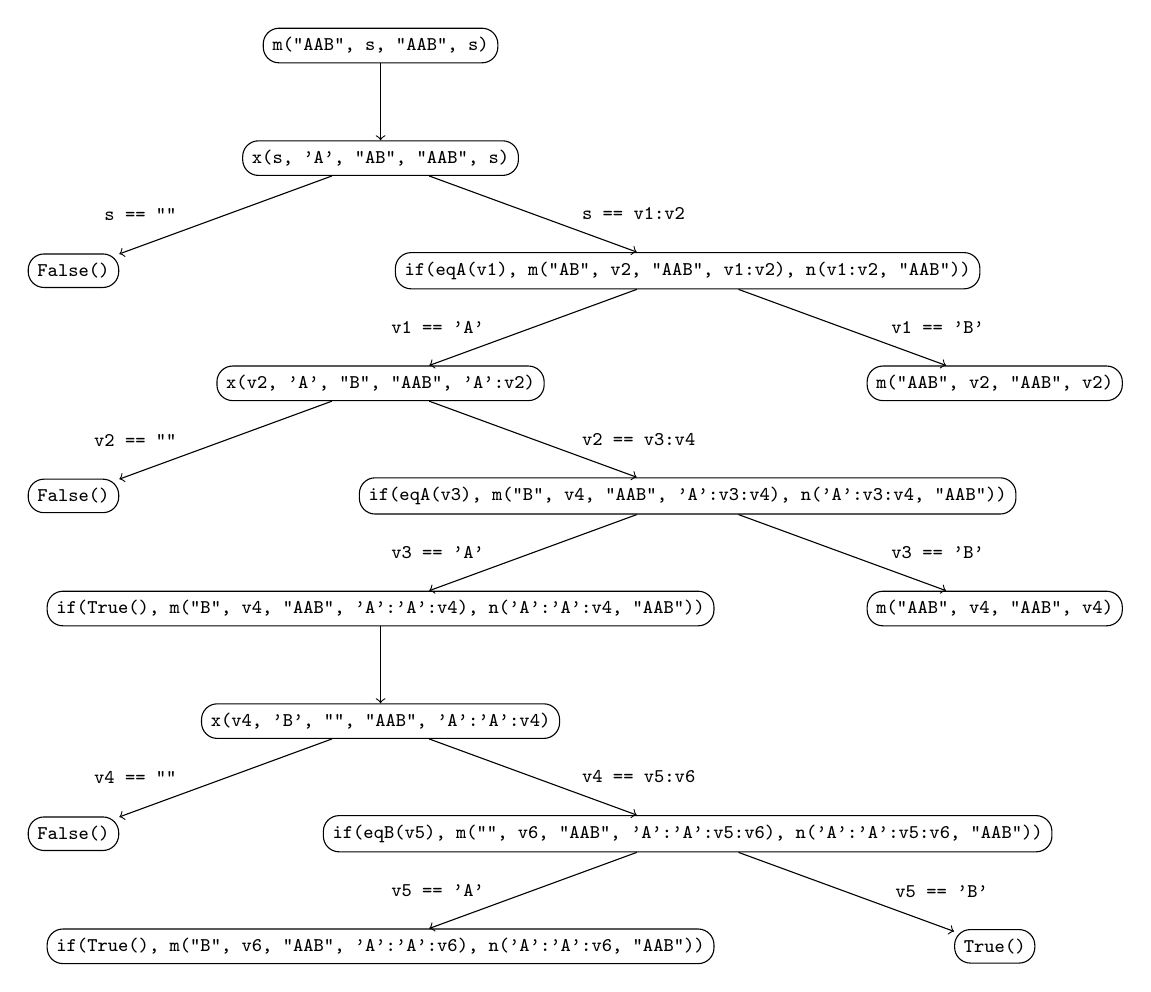
\begin{tikzpicture}[scale=1.3,
level distance=11mm,
level/.style={sibling distance=60mm},
conf/.style={
	rectangle,minimum width=10mm,minimum height=4mm,rounded corners=2mm,
	draw=black,
	font=\ttfamily\scriptsize},
label/.style={font=\ttfamily\scriptsize}
]
% \tikzstyle{level 2}=[sibling distance=45mm]
% \tikzstyle{level 3}=[sibling distance=45mm]
% \tikzstyle{level 4}=[sibling distance=22mm]
% \tikzstyle{level 5}=[sibling distance=70mm]
% \tikzstyle{level 6}=[sibling distance=30mm]
% \tikzstyle{level 7}=[sibling distance=30mm]
% \tikzstyle{level 8}=[sibling distance=30mm]
% \tikzstyle{level 9}=[sibling distance=30mm]
% \tikzstyle{level 10}=[sibling distance=30mm]
\node[conf]{m("AAB", s, "AAB", s)}
child[->]{node[conf]{x(s, 'A', "AB", "AAB", s)}
child[->]{node[conf]{False()}
edge from parent node[left,label,xshift=-5mm]{s == ""}}
child[->]{node[conf]{if(eqA(v1), m("AB", v2, "AAB", v1:v2), n(v1:v2, "AAB"))}
child[->]{node[conf]{x(v2, 'A', "B", "AAB", 'A':v2)}
child[->]{node[conf]{False()}
edge from parent node[left,label,xshift=-5mm]{v2 == ""}}
child[->]{node[conf]{if(eqA(v3), m("B", v4, "AAB", 'A':v3:v4), n('A':v3:v4, "AAB"))}
child[->]{node[conf]{if(True(), m("B", v4, "AAB", 'A':'A':v4), n('A':'A':v4, "AAB"))}
child[->]{node[conf]{x(v4, 'B', "", "AAB", 'A':'A':v4)}
child[->]{node[conf]{False()}
edge from parent node[left,label,xshift=-5mm]{v4 == ""}}
child[->]{node[conf]{if(eqB(v5), m("", v6, "AAB", 'A':'A':v5:v6), n('A':'A':v5:v6, "AAB"))}
child[->]{node[conf]{if(True(), m("B", v6, "AAB", 'A':'A':v6), n('A':'A':v6, "AAB"))}
edge from parent node[left,label,xshift=-5mm]{v5 == 'A'}}
child[->]{node[conf]{True()}
edge from parent node[right,label,xshift=5mm]{v5 == 'B'}}
edge from parent node[right,label,xshift=5mm]{v4 == v5:v6}}}
edge from parent node[left,label,xshift=-5mm]{v3 == 'A'}}
child[->]{node[conf]{m("AAB", v4, "AAB", v4)}
edge from parent node[right,label,xshift=5mm]{v3 == 'B'}}
edge from parent node[right,label,xshift=5mm]{v2 == v3:v4}}
edge from parent node[left,label,xshift=-5mm]{v1 == 'A'}}
child[->]{node[conf]{m("AAB", v2, "AAB", v2)}
edge from parent node[right,label,xshift=5mm]{v1 == 'B'}}
edge from parent node[right,label,xshift=5mm]{s == v1:v2}}}


;

\end{tikzpicture}

%Просто граф.

%\newpage
\begin{tikzpicture}[scale=1.3,
level distance=11mm,
level/.style={sibling distance=60mm},
conf/.style={
	rectangle,minimum width=10mm,minimum height=4mm,rounded corners=2mm,
	draw=black,
	font=\ttfamily\scriptsize},
label/.style={font=\ttfamily\scriptsize},
base/.style={
	rectangle split, rectangle split parts=2, draw,rounded corners=2mm,
	draw=black,
	font=\ttfamily\scriptsize},
]
% \tikzstyle{level 2}=[sibling distance=45mm]
% \tikzstyle{level 3}=[sibling distance=45mm]
% \tikzstyle{level 4}=[sibling distance=22mm]
% \tikzstyle{level 5}=[sibling distance=70mm]
% \tikzstyle{level 6}=[sibling distance=30mm]
% \tikzstyle{level 7}=[sibling distance=30mm]
% \tikzstyle{level 8}=[sibling distance=30mm]
% \tikzstyle{level 9}=[sibling distance=30mm]
% \tikzstyle{level 10}=[sibling distance=30mm]
\node[base,red]{m("AAB", s, "AAB", s)\nodepart{second}f1(s)}
child[->]{node[base]{x(s, 'A', "AB", "AAB", s)\nodepart{second}g2(s)}
child[->]{node[conf]{False()}
edge from parent node[left,label,xshift=-5mm]{s == ""}}
child[->]{node[base]{if(eqA(v1), m("AB", v2, "AAB", v1:v2), n(v1:v2, "AAB"))
\nodepart{second}g3(v1, v2)}
child[->]{node[base]{x(v2, 'A', "B", "AAB", 'A':v2)
\nodepart{second}g4(v2)}
child[->]{node[conf]{False()}
edge from parent node[left,label,xshift=-5mm]{v2 == ""}}
child[->]{node[base]{if(eqA(v3), m("B", v4, "AAB", 'A':v3:v4), n('A':v3:v4, "AAB"))
\nodepart{second}g5(v3, v4)}
child[->]{node[base,blue]{if(True(), m("B", v4, "AAB", 'A':'A':v4), n('A':'A':v4, "AAB"))
\nodepart{second}f6(v4)}
child[->]{node[base]{x(v4, 'B', "", "AAB", 'A':'A':v4)
\nodepart{second}g7(v4)}
child[->]{node[conf]{False()}
edge from parent node[left,label,xshift=-5mm]{v4 == ""}}
child[->]{node[base]{if(eqB(v5), m("", v6, "AAB", 'A':'A':v5:v6), n('A':'A':v5:v6, "AAB"))
\nodepart{second}g8(v5, v6)}
child[->]{node[base,blue]{if(True(), m("B", v6, "AAB", 'A':'A':v6), n('A':'A':v6, "AAB"))
\nodepart{second}f6(v6)}
edge from parent node[left,label,xshift=-5mm]{v5 == 'A'}}
child[->]{node[conf]{True()}
edge from parent node[right,label,xshift=5mm]{v5 == 'B'}}
edge from parent node[right,label,xshift=5mm]{v4 == v5:v6}}}
edge from parent node[left,label,xshift=-5mm]{v3 == 'A'}}
child[->]{node[base,red]{m("AAB", v4, "AAB", v4)
\nodepart{second}f1(v4)}
edge from parent node[right,label,xshift=5mm]{v3 == 'B'}}
edge from parent node[right,label,xshift=5mm]{v2 == v3:v4}}
edge from parent node[left,label,xshift=-5mm]{v1 == 'A'}}
child[->]{node[base,red]{m("AAB", v2, "AAB", v2)
\nodepart{second}f1(v2)}
edge from parent node[right,label,xshift=5mm]{v1 == 'B'}}
edge from parent node[right,label,xshift=5mm]{s == v1:v2}}};
\end{tikzpicture}

In the last figure we again mark by the same color nodes, which are equal
up to renaming.
The upper part of each node contains the original configuration,
the lower part -- the new configuration generated by \texttt{res}.

\begin{lstlisting}[style=demo,escapechar=!]
ghci> let g = ...

-- demo24
ghci> residuate g
f1(s)
f1(s) = g2(s);
g2("") = False();
g2(v1:v2) = g3(v1, v2);
g3('A', v2) = g4(v2);
g3('B', v2) = f1(v2);
g4("") = False();
g4(v3:v4) = g5(v3, v4);
g5('A', v4) = f6(v4);
g5('B', v4) = f1(v4);
f6(v4) = g7(v4);
g7("") = False();
g7(v5:v6) = g8(v5, v6);
g8('A', v6) = f6(v6);
g8('B', v6) = True();
\end{lstlisting}